% --------------------------------------------------------------
% This is all preamble stuff that you don't have to worry about.
% Head down to where it says "Start here"
% --------------------------------------------------------------
 
\documentclass[12pt]{article}
 
\usepackage[margin=1in]{geometry} 
\usepackage{amsmath,amsthm,amssymb, graphicx, verbatim}
 \usepackage{algorithm}
\usepackage{algorithmic}

\newcommand{\N}{\mathbb{N}}
\newcommand{\Z}{\mathbb{Z}}
 
\newenvironment{theorem}[2][Theorem]{\begin{trivlist}
\item[\hskip \labelsep {\bfseries #1}\hskip \labelsep {\bfseries #2.}]}{\end{trivlist}}
\newenvironment{lemma}[2][Lemma]{\begin{trivlist}
\item[\hskip \labelsep {\bfseries #1}\hskip \labelsep {\bfseries #2.}]}{\end{trivlist}}
\newenvironment{exercise}[2][Exercise]{\begin{trivlist}
\item[\hskip \labelsep {\bfseries #1}\hskip \labelsep {\bfseries #2.}]}{\end{trivlist}}
\newenvironment{problem}[2][Problem]{\begin{trivlist}
\item[\hskip \labelsep {\bfseries #1}\hskip \labelsep {\bfseries #2.}]}{\end{trivlist}}
\newenvironment{question}[2][Question]{\begin{trivlist}
\item[\hskip \labelsep {\bfseries #1}\hskip \labelsep {\bfseries #2.}]}{\end{trivlist}}
\newenvironment{corollary}[2][Corollary]{\begin{trivlist}
\item[\hskip \labelsep {\bfseries #1}\hskip \labelsep {\bfseries #2.}]}{\end{trivlist}}

\newenvironment{solution}{\begin{proof}[Solution]}{\end{proof}}
 
\begin{document}
 
% --------------------------------------------------------------
%                         Start here
% --------------------------------------------------------------
 
\begin{comment} 
Please include a section in your report detailing your GPU implementation, as well as its performance over varying numbers of particles. Here is the list of items you might show in your report:

A plot in log-log scale that shows the performance of your code versus the naive GPU code
A plot of the speedup of the GPU code versus the serial, openmp, mpi runs on the CPU of the node
A description of any synchronization needed
A description of any GPU-specific optimizations you tried
A discussion on the strengths and weaknesses of CUDA and the current GPU architecture
\end{comment}

\title{CS 267 Homework 2 Part 3}
\author{Xingyou Song \footnote{xsong@berkeley.edu - Xingyou wrote the report, presented techniques and strategies for optimization, and coded some parts}, Yao Yuan \footnote{yao\_yuan@berkeley.edu - Yao coded a significant part of the code in C and tested using various compiler settings}, Jingbo Wu\footnote{wu622@berkeley.edu - Jingbo mainly contributed to the report and coding.}} %replace with your name
\date{March 9, 2018} 
\maketitle

\section{Old Algorithm (Serial)}
Recall from our previous part 1 submission that we used the following method to achieve $O(n)$ time: Our technique was to separate the space (formed by the bounding box of the entire set of points), into a grid of $G \times G$ blocks, where $G$ is the partition number of each of the x or y dimensions. Let $n$ be the number of particles in the simulation. For our serial implementation, $G = n$, while in our parallel implementation, $G = \sqrt{n}$. (For these two cases, they are also set as the particle interaction minimum distance, in case the grids are too small). Then for any neighboring blocks, we brute-forced the force computations over the union of the particles. \\\\
The order then follows: 
\begin{itemize}
  \item For each block, compute inner forces within the block.
  \item For each block, compute the forces of its particles affected by the block's 8 neighbors.
  \item Move all of the particles as needed. 
\end{itemize}

\subsection{Proof of Concept} In the serial setting, in every stride interval (1-dimensional) of other the x or y axis, there is an average of 1 point. The idea here is to shortcut the force-checking process by only brute-force calculating forces in between neighboring blocks.  More rigorously, suppose we assume that each of the $n$ particles has uniform probability to be placed in one of the $n \times n$ blocks. Our total calculation will then be $$\sum_{neighboring blocks A, B}  brute\_force(A, B)$$ where the runtime of $brute\_force(A,B)$ is $|A||B|$ to brute force all of the points' forces. Note that by linearity of expectation, we may then consider the expected total calculation as $$O(n^{2}) \mathbb{E} \left[brute\_force(A,B) \right]$$
After some calculation, we find that $\mathbb{E} \left[brute\_force(A,B) \right] \le O(1/n)$ which implies the linearity result. 

\section{GPU/CUDA Modifications}

\subsection{Ordinary Implementation}
In the global memory updating solution, we allow each block in the particle space (renamed "bins" in the code) of the grid to correspond to each thread on the GPU. Every physical GPU block corresponds to a $1 \times k$ tile on the grid, where $k$ is the blockDimension.x (i.e max number of threads on a block). Every thread would simulate/compute in its bin. However, for location updating, we then updated a global memory (called redundantBins in the code) so that particles from bin A go to bin B from time $t$ to $t+1$. The next time step would load the global memory back into the GPU again. Thus, every loop iteration consists of the following:

\begin{itemize}
\item Load from redundantBins (global memory) into corresponding GPU blocks. 
\item Each thread computes the particles' forces and new locations in the thread's corresponding bin. 
\item (Synchronize all threads first) Send particles to the corresponding positions in the redundantBins for next iteration. 
\item Repeat. 
\end{itemize}

\subsection{Possible Improvements}
Note that there are some flaws with this approach that could or cannot be improved:
\begin{itemize}
\item The global memory updating scheme is a large overhead, as we're making 2 reads of the entire grid memory at every time step.

\item Rather than each GPU block representing a $1 \times k$ tile, A block might represent a $\sqrt{k} \times \sqrt{k}$ tile instead, because this requires fewer memory operations for each GPU block. (i.e. the perimeter of this square is $O(\sqrt{k})$, rather than the $O(k)$ from the $1 \times k$ tile. However, this method is very coding intensive (we attempted to do so, but there are an incredibly large number of edge cases related to computing indices), because CUDA memory copying is inherently sequential. 

\item Also, this square-tiling approach does not actually remove the global memory updating scheme cleanly (but can improve a few memory updates), because it doesn't help with the case when a particle has an extremely large speed that forces it to jump between very far bins on the grid. Since CUDA doesn't allow inter-block communication, (e.g. we can't just tell thread A corresponding to a high speed particle in bin A, to communicate with thread B to collect that particle into bin B in the next time step, using their corresponding blocks), global updating seems to be needed. 

\item We are not utilizing shared memory for threads on the same block - this means that for a $1 \times k$ block, every thread accesses its 8 neighbors, with some accesses shared between threads (for a total of $8k$ global reads) In order to fix this, we propose preloading all of the neighbors (and itself) for a shared memory for the $3 \times (k+2)$ "perimeter tile" covering the original tile. This would give us $3(k+2)$ global reads, and $8k$ shared memory reads instead. Since shared memory is on the order of $100$ times faster than global memory, theoretically we should achieve $8*100/(3*100 + 8) = 2.59$x speedup for memory reads. For $\sqrt{k} \times \sqrt{k}$ blocking, the naive memory approach would give us $8k$ global reads again, and the local memory optimization would give us $(\sqrt{k}+2)^{2}$ global memory reads with $8k$ shared memory reads instead, which should achieve $8*100/(100 + 8) = 7.4$ times memory speedup.  
\end{itemize}
\subsection{Attempted Improvements}
\begin{itemize}
\item We coded a 2d version of the blocking procedure, using $\sqrt{k} \times \sqrt{k}$ GPU blocks. However, this actually resulted in a slightly slower performance. This is possibly due to lack of cache use in this implementation, as well as more overheads from computing correct indices. 
\item We coded a version of shared memory for the $\sqrt{k} \times \sqrt{k}$ block case, but found that it this was even impossible due to hardware limitations even for $k = 64$ threads. This is because of the small size of the shared memory in the GPU. Furthermore, we suspect that while theoretically if this were allowed, the overhead from the if-statements needed from computing correct indices between global memory and shared local memory would drastically affect performance as well.  
\end{itemize}
\newpage 
\subsection{Results}
\begin{figure}[h]
  \caption{GPU Final Code vs GPU naive (Avg Speed up 35.29, GPU final log-log slope avg is 0.20}
  \centering 
  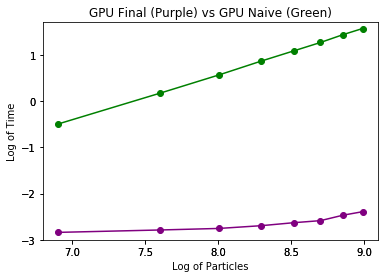
\includegraphics[width = 0.65\textwidth]{GPU_final_vs_GPU_naive.png}
  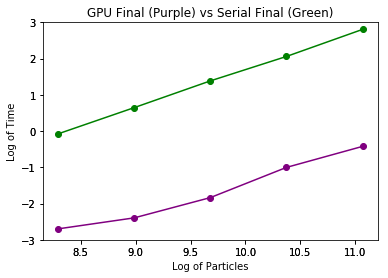
\includegraphics[width = 0.65\textwidth]{GPU_final_vs_Serial_final.png}
\end{figure}
Note that as we have more particles, we have slightly lower slope for our GPU-final code, while serial and GPU-naive codes' slopes are very consistent. 
\newpage 
\subsubsection{Comparison to Other Parallelism}

\begin{figure}[h]
  \caption{Performance for Serial, MPI 32 Threads, OpenMP 32 Threads, GPU}
  \centering 
  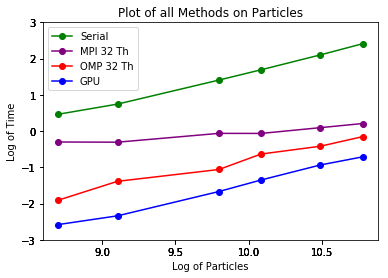
\includegraphics[width = 0.65\textwidth]{serial_mpi_openmp_gpu.png}
\end{figure}
We found that ultimately, the GPU still worked better than the 32-threaded MPI and OpenMP versions, for particle sizes (6000-48000). It is likely that from viewing the slopes of the curves, the GPU will remain the fastest, although MPI may overtake OpenMP for larger particle sizes. \footnote{We did not simulate more due to overloading the XSEDE allocation - our wait time went to 80 hours for a batch job.}

\subsection{Strengths and Weaknesses of CUDA}
\subsubsection{Strengths}
CUDA allows for very large parallel memory reads, which makes it suitable for when there are a massive amount of particles (we're able to simulate orders of magnitude more particles than other frameworks), unlike MPI, which is limited by a memory reading bandwidth. It also allows for a significant number of threads to run, which also increases parallelism. 


\subsubsection{Weaknesses}
The problem of communication in the GPU is one of the greatest limitations - unlike MPI, there is no good method of allowing different GPU blocks to communicate with each other than merely copying back and forth between global memory, which makes it ineffective for computations that require shared resources. This also means that topology in a problem can't be exploited (i.e. the $\sqrt{k} \times \sqrt{k}$ doesn't actually get much speedup even if we've reduced the order of the perimeter sums). Lastly, as we've seen from the hardware limitation, we realized that the cache size for each block is actually quite small and doesn't scale as well as the number of threads allowed.



\begin{comment}
\section{Results}
We present our results (every processor only has one thread): 

\begin{table}[h]

\begin{tabular}{||c c c||} 
 \hline
 Particles & Avg Strong Scaling & Avg Weak Scaling  \\ [0.5ex] 
 \hline\hline 
 %%%%%%%%%%
 500 & 0.27 & 0.49 \\
 \hline 
 1000 & 0.31 & 0.40 \\
 \hline 
 1500 & 0.31 & 0.41  \\
 \hline
%%% DO NOT TOUCH PLS 
\end{tabular}

\end{table}
\begin{table}[h]

 \begin{tabular}{||c c c||} 
 \hline
 Particles & Processor & Time (s)  \\ [0.5ex] 
 \hline\hline
 500 & (Serial) & 0.081663 \\
 \hline 
 500 & 1 & 0.095706  \\
 \hline
  500 & 2 & 0.07736  \\
 \hline
  500 & 4 & 0.104709  \\
 \hline
  500 & 6 & 0.078448  \\
 \hline
  500 & 12 & 0.107769  \\
 \hline
  500 & 16 & 0.080899  \\
 \hline
  500 & 24 & 0.104492   \\
 \hline
  500 & 32 & 0.096736  \\
 \hline
  1000 & 2 & 0.129597  \\
 \hline
  2000 & 4 & 0.237802  \\
 \hline
  3000 & 6 & 0.232805  \\
 \hline
  6000 & 12 & 0.362595  \\
 \hline
  8000 & 16 & 0.504432  \\
 \hline
  12000 & 24 & 0.520144  \\
 \hline
 %%%%%%%%%%%%%
%%% DO NOT TOUCH PLS 
\end{tabular}
\begin{tabular}{||c c c||} 
 \hline
 Particles & Processor & Time (s)  \\ [0.5ex] 
 \hline\hline 
 %%%%%%%%%%%%%
 1000 & (Serial) & 0.169638 \\
 \hline 
 1000 & 1 & 0.183064 \\
 \hline 
 1000 & 2 & 0.129295 \\
 \hline  
 1000 & 4 & 0.128382 \\
 \hline 
 1000 & 6 & 0.121484 \\ 
 \hline  
 1000 & 12  & 0.121381 \\
 \hline 
 1000 & 16 & 0.120848 \\ 
 \hline  
 1000 & 24 & 0.133204 \\
 \hline 
 1000 & 32 &  0.13395 \\ 
 \hline 
 2000 & 2 & 0.249004 \\
 \hline 
 4000 & 4 & 0.379472 \\
 \hline 
 6000 & 6 & 0.690608 \\ 
 \hline 
 12000 & 12 & 0.635974 \\
 \hline 
 16000 & 16 & 0.70321 \\
 \hline 
 24000 & 24 & 0.810816 \\
 \hline 
 32000 & 32 & 0.842401 \\
 \hline 
 %%%%%%%%%%

%%% DO NOT TOUCH PLS 
\end{tabular}
\end{table}
\begin{table}
\begin{tabular}{||c c c||} 
 \hline
 Particles & Processor & Time (s)  \\ [0.5ex] 
 \hline\hline 
 %%%%%%%%%%
 1500 & (Serial) & 0.25489 \\
 \hline 
 1500 & 1 & 0.284891 \\
 \hline 
 1500 & 2 & 0.196361  \\
 \hline  
 1500 & 4 & 0.183619 \\
 \hline 
 1500 & 6 & 0.164744  \\ 
 \hline  
 1500 & 12  & 0.139465 \\
 \hline 
 1500 & 16 & 0.158564  \\ 
 \hline  
 1500 & 24 &  0.14834 \\
 \hline 
 1500 & 32 &  0.169517 \\ 
 \hline 
 3000 & 2 & 0.369944  \\
 \hline 
 6000 & 4 &  0.739809  \\
 \hline 
 9000 & 6 & 0.736118 \\ 
 \hline 
 18000 & 12 & 0.938799 \\
 \hline 
 24000 & 16 & 0.937171 \\
 \hline 
 36000 & 24 & 1.09924 \\
 \hline 
 48000 & 32 & 1.23157  \\
 \hline 
%%% DO NOT TOUCH PLS 
\end{tabular}

\end{table} 

\clearpage 

\subsection{Performance}
Note that when we fix the particle size and vary the number of processors, the curve becomes slightly smoother. At 500 points, we see that there is no clear sign of monotonicity, while at 1500 points, we see that our performance increases as the number of processors increases, but performance decreases at 20-32 processors. We seem to only see the $O(n/p)$ performance when the number of processors is between 5-15. This shows that communication overhead becomes a significant factor in designing the simulation. 
\\ \\ 
However, when we vary the number of particles with the number of processors, our performance becomes asymptotic as the time seems to be reaching an asymptotic limit - This suggests that for both large $n$ and $p$, we are also reaching a $O(n/p)$ asymptotic performance. Since at 1500 particles/processor, the log of time slightly increases, this means that there is a slight dominance of the number of particles - e.g. our asymptotic time could possibly be more similar to $O(n^{1 + \epsilon}/p)$ where $\epsilon > 0$, which makes sense as more particles imply more boundary changes, which implies more memory communication between processors, which has a much worse performance scaling than pure computation. 
\clearpage 

\begin{figure}[h]
  \caption{Fixed Particle Sizes, Varying Processor}
  \centering 
  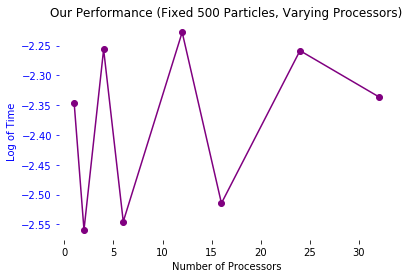
\includegraphics[width = 0.65\textwidth]{500_fixed_particles_varying_processor.png}
  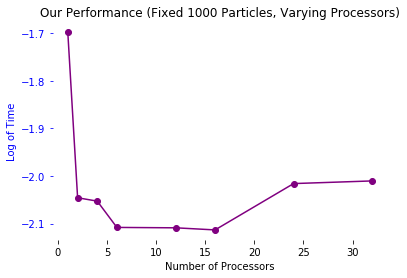
\includegraphics[width = 0.65\textwidth]{1000_fixed_particles_varying_processor.png}
  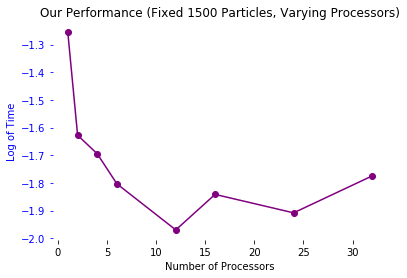
\includegraphics[width = 0.65\textwidth]{1500_fixed_particles_varying_processor.png}
\end{figure}


\begin{figure}[h]
  \caption{Varying Particle Size with Processor}
  \centering
    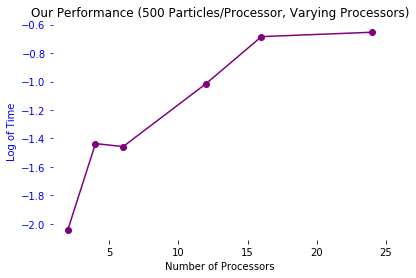
\includegraphics[width = 0.65\textwidth]{500_varying_particles_varying_processor.png}
  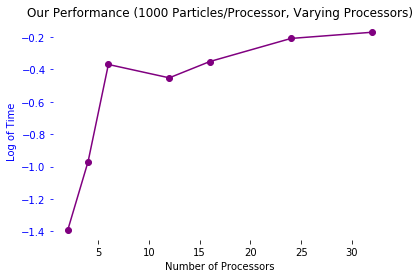
\includegraphics[width = 0.65\textwidth]{1000_varying_particles_varying_processor.png}
  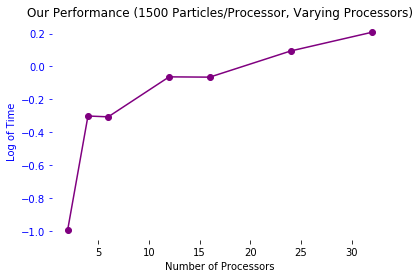
\includegraphics[width = 0.65\textwidth]{1500_varying_particles_varying_processor.png}
 
\end{figure}

\clearpage
\subsection{Doing Better?}
We attempted other variants of MPI, including as mentioned, different shapes for the "sector" used by each processor. We may possibly see different results if, for example, processors which are assigned to the outer blocks of the grid are larger, specifically because particles bounce back from the wall on the outer edge, requiring less communication. 
\\ \\
Another optimization considered is the communication architecture used as well - we found that including a master processor which controls the synchronization of the worker processors resulted in a slow down. It is possible that we could, instead of enforcing every worker processor to signal all of the other worker processors its completion, we divide the grid into e.g. 2 groups, with 2 masters - this way all processors belonging to a group may only signal his completion to the corresponding master, and allow synchronization between the two masters. This setting would be more appropriate for 2 dense regions that are not connected well. 
% --------------------------------------------------------------
%     You don't have to mess with anything below this line.
% --------------------------------------------------------------
 \end{comment}
\end{document}
